


\subsection{A customer successfully purchases gas and charges it on
a monthly bill}

The sequence diagram is showing on fig~\ref{fig:seq-diagram1}

\subsection{A customer purchases gas and attempts to pay by credit
card but his card is refused. He then pays by cash to the cashier.}

The sequence diagram is showing on fig~\ref{fig:seq-diagram2}

\subsection{The cashier successfully processes a monthly payment by
credit card.}

The sequence diagram is showing on fig~\ref{fig:seq-diagram3}


\begin{landscape}
\begin{figure}[!h]
\centering
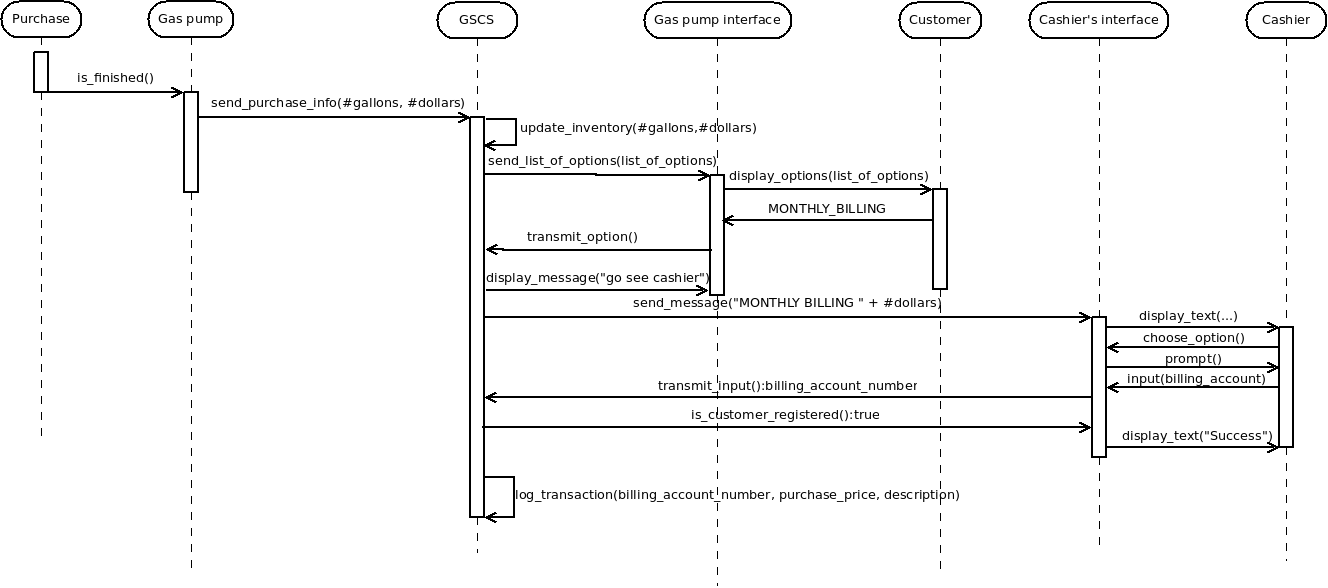
\includegraphics[width=\linewidth]{drafts/sequence_1.png}
\caption{Class diagram}
\label{fig:seq-diagram1}
\end{figure}
\end{landscape}

\begin{landscape}
\begin{figure}[!h]
\centering
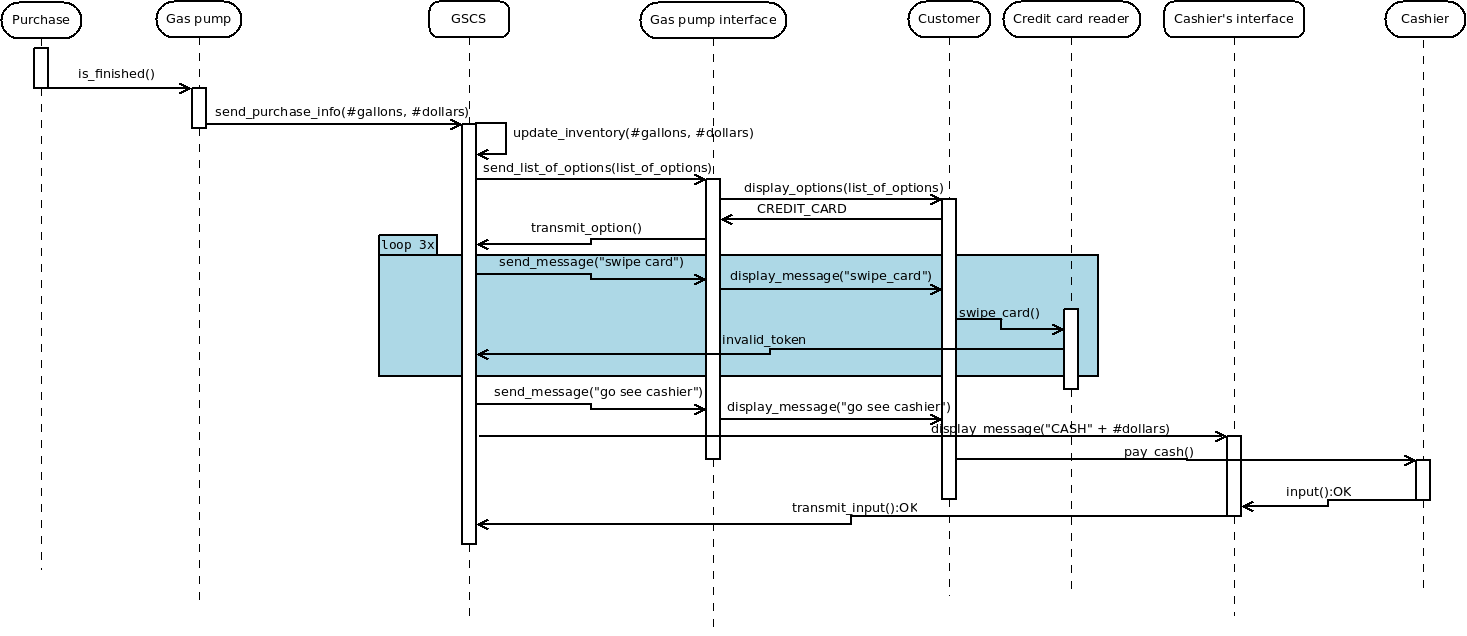
\includegraphics[width=\linewidth]{drafts/sequence_2.png}
\caption{Class diagram}
\label{fig:seq-diagram2}
\end{figure}
\end{landscape}

\begin{landscape}
\begin{figure}[!h]
\centering
%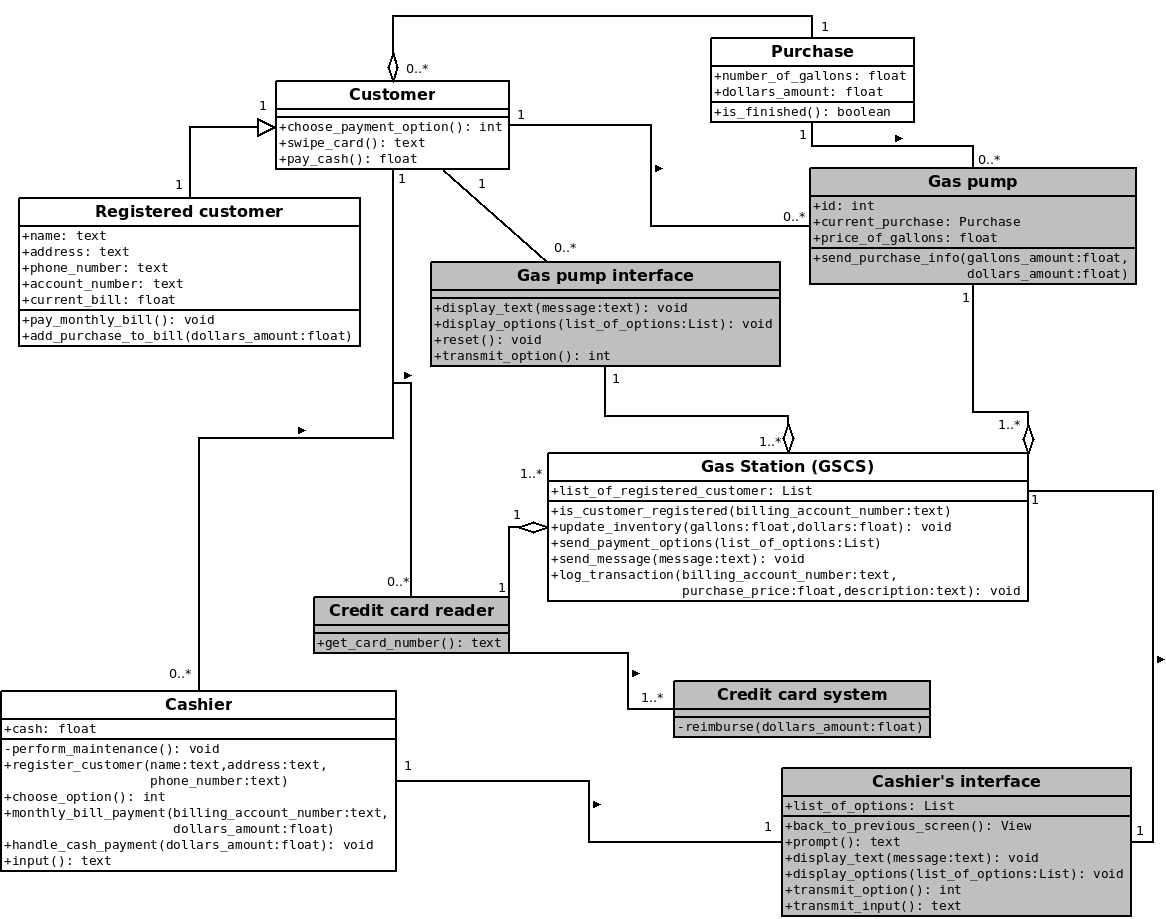
\includegraphics[width=\linewidth]{drafts/class_diagram.png}
\caption{Class diagram}
\label{fig:seq-diagram3}
\end{figure}
\end{landscape}

